\subsection{Leg detection} \label{sec:LegDetect}
Leg detection is used to calculate the geometry of legs and apply these calculation in a way so that a person's centre can be found. An overview can be viewed in figure \ref{fig:legflow}.
\begin{figure}[H]
    \centering
    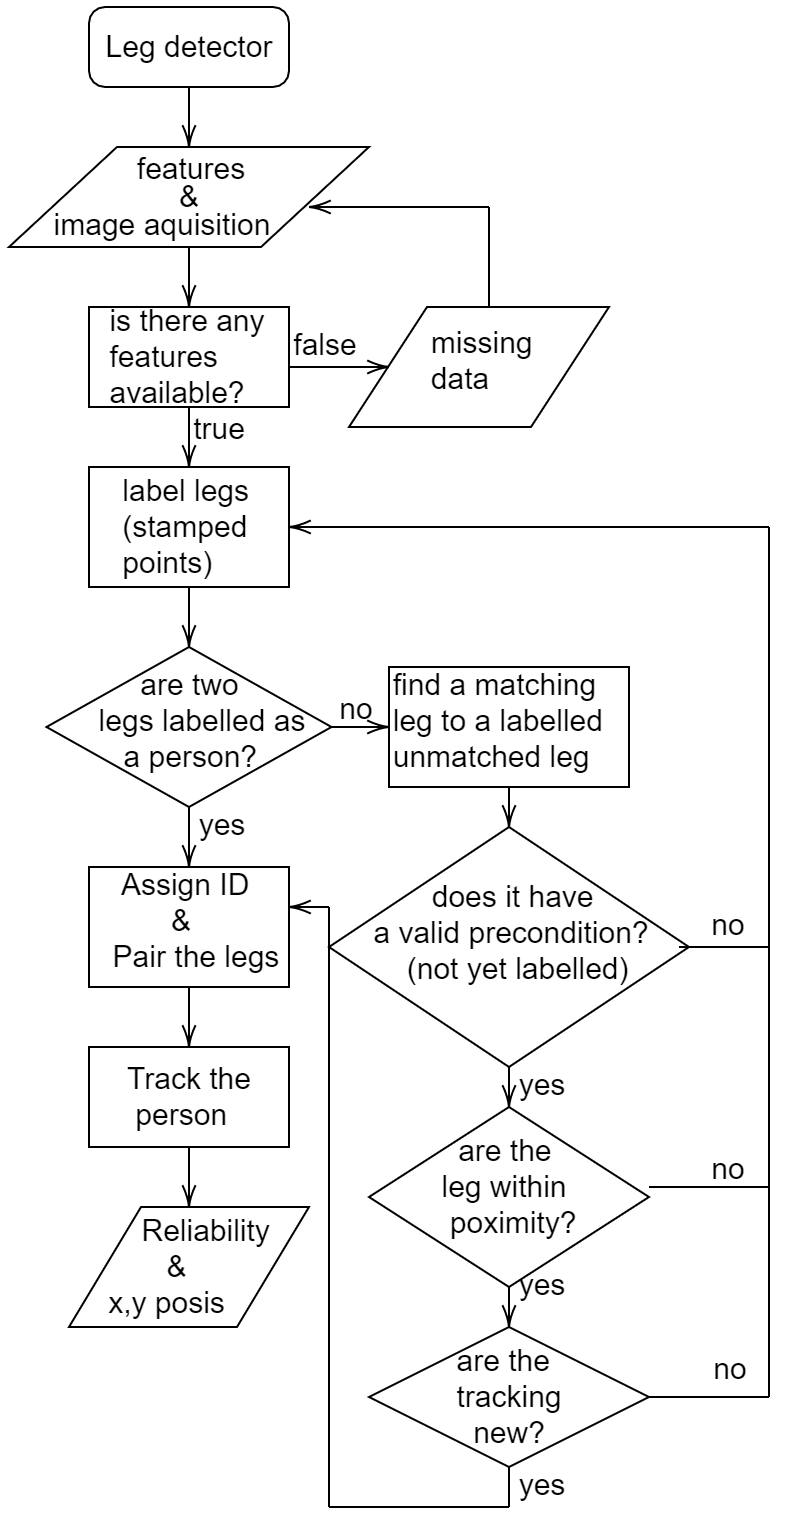
\includegraphics[width=.6\textwidth]{figures/leg2.png}
    \caption{Overview of the leg detection algorithm}
    \label{fig:legflow}
\end{figure}

%features:
The leg detector converts a number of points, or clusters, in the image into readable matrices for the OpenCV program. These matrices are then used to identify features, which is used to determine the reliability for the leg detection. Some of the features are:

\begin{itemize}
    \item Circularity
    \item Width
    \item Radius
    \item Mean angular distances
\end{itemize}

The reliability decides whether the tracked object is a person or not. These features establishes the foundation of a single leg and later on in the algorithm these legs are paired to connect them as persons. However, two table-legs can also be tracked but the width and radius often makes them displayed as false-positives, which will appear as blue dots when the tracker is visualised in RViz. And the people detected as persons will appear as a green dot with 2 red dots on each side, which is the legs as seen in figure \ref{fig:rviz}. RViz is a tool used to run visualisation of a robot.\\

\begin{figure}[H]
    \centering
    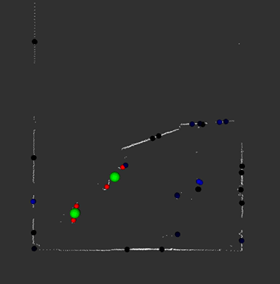
\includegraphics[width=0.8\textwidth, height=10cm]{figures/rviz.png}
    \caption{Visualisation of the leg detection in RViz. The dark-blue dots are false-positives and the green dots are perceived as humans, while the red dots are perceived as legs}
    \label{fig:rviz}
\end{figure}

In this algorithm there is 3 files worth mentioning, the first is the training.cpp. This file includes the data read from the camera and it tries to continuously classify the different aforementioned features so that the code can keep running. However the training.cpp is also continuously trying to reduce the computational power, much like the HAAR cascade, see section \ref{sec:Face}, by only looking for the aforementioned clusters. If only false-positives or no clusters is in the LIDARs field of view the code will only run this section of the code and the computation is reduced.\\
The second file is the feature\_extraction.cpp, which has briefly been touched upon by stating which features it scans for and how the points gathered from the LIDAR is converted to a readable matrix to use with OpenCV.\\
The third file is the leg\_detector.cpp and this file is where the actual leg detection happens. A combination of geometry messages and tracking of the leg is implemented in this file. However the first thing to establish is that each leg is provided with a time-stamp when it has been tracked and this time-stamp will serve as constant in a function that measures the walking patterns or speed of the tracked humans.\\
The leg\_detector algorithm tracks people by following a single rule for the legs, the distance between the legs. An estimate of the average distance between the legs of a person has been found and the writers of the algorithm has established that this number is between 20 to 50cm. When each feature has been reasonably close to resemblance of a leg the tracker stamps it and then it continuously looks for other legs in the perimeter of 20 to 50cm. If another leg is found it will ID these legs as person and the readings of the leg detector will be published so that position, time-stamps, IDs, and reliability, etc. can be surveilled, as seen in figure \ref{fig:reliability}.

\begin{figure}[H]
    \centering
    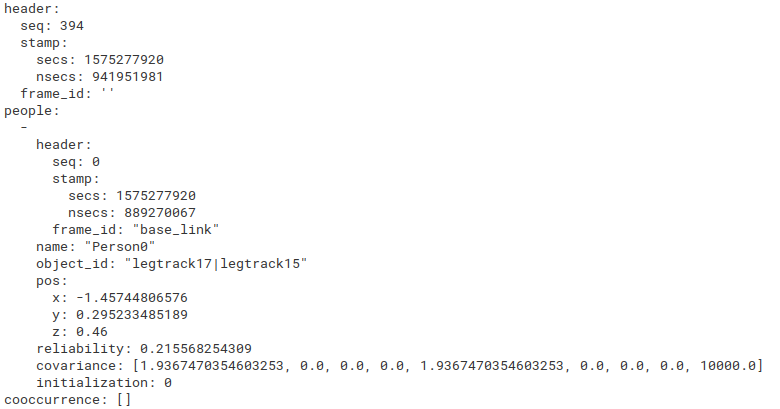
\includegraphics[width=\textwidth]{figures/leg_detector_msg.png}
    \caption{The message structure of the leg detection, published on the topic /legdetector}
    \label{fig:reliability}
\end{figure}

However one measurement is not mentioned and that is the covariance. The covariance is an array that utilises geometry messages to establish the relations between the values of the position messages and that of the reliability score. In the position messages the authors of the code include several measured values to get a reasonable covariance value. %line 880 in the code
With these detection measurements available human legs can be tracked and connected with the aforementioned face-id.\\